\documentclass[10pt]{beamer}

\usepackage{tikz}
\usetikzlibrary{positioning,shapes,shadows,arrows}
\tikzstyle{abstract}=[rectangle, rounded corners, draw=black, anchor=north, fill=blue!10, text centered, minimum height={height("Gp")+2pt}, minimum width=3cm, font=\footnotesize]

\definecolor{links}{HTML}{0000CC}
\hypersetup{colorlinks,linkcolor=,urlcolor=links}

\mode<handout>
{
  \usepackage{pgfpages}
  \pgfpagesuselayout{4 on 1}[a4paper,border shrink=3mm,landscape]
  \usetheme{CambridgeUS}
  \usecolortheme{lily}
}

\mode<beamer>
{
  \usetheme{CambridgeUS}
}

\AtBeginSection[]
{
  \begin{frame}
    \frametitle{Outline}
    \tableofcontents[currentsection]
  \end{frame}
}

\setbeamerfont{frametitle}{family=\rmfamily,series=\bfseries,size={\fontsize{10}{10}}}
\setbeamertemplate{frametitle continuation}[from second]

\title{Dynare Time Series \& Reporting}
\author{Houtan Bastani}
\institute{CEPREMAP}
\date{13 June 2014}

\begin{document}

\begin{frame}
  \titlepage
\end{frame}

\begin{frame}[t]
  \frametitle{Outline}
  \tableofcontents
\end{frame}

%
% DATES
%
\section{Time Series}

\subsection{Overview}
\begin{frame}[fragile,t]
  \frametitle{Overview}
  \begin{itemize}
  \item Provide support for time series in Dynare
  \item Introduced in Dynare 4.4
  \item Currently only used for reporting
  \item Use will increase with time (\textit{e.g.,} to be included in new estimation code)
  \item NB: More complete information is included in the Dynare manual
  \end{itemize}
\end{frame}


\subsection{Syntax}
\begin{frame}[fragile,t]
  \frametitle{Syntax}
  \begin{itemize}
  \item Two components of a time series:
    \begin{itemize}
    \item A time component. In Dynare: \texttt{dates}
    \item A data component mapped to time. In Dynare: \texttt{dseries}
    \end{itemize}
  \end{itemize}
\end{frame}

\subsubsection{\texttt{dates} Syntax}
\begin{frame}[fragile,t]
  \frametitle{\texttt{dates} Syntax}
  \begin{itemize}
  \item The \texttt{dates} command creates an object that represents at least one date at a given frequency
    \begin{itemize}
    \item Yearly: \texttt{`Y', `y', 1}
    \item Quarterly: \texttt{`Q', `q', 4}
    \item Monthly: \texttt{`M', `m', 12}
    \item Weekly: \texttt{`W', `w', 52}
    \end{itemize}
  \item It has two slightly different syntaxes
    \begin{itemize}
    \item One for inclusion in \texttt{.m} files
    \item One for inclusion in \texttt{.mod} files (simplified using the preprocessor)
      \begin{itemize}
        \item To prevent date translation, escape the date with `\texttt{\$}' (\textit{e.g.,} \texttt{\$2020y})
      \end{itemize}
    \end{itemize}
  \item Minimal restrictions on dates. Can be
    \begin{itemize}
      \item Negative
      \item Empty
      \item Noncontiguous
    \end{itemize}
  \item Can index a \texttt{dates} object. If \texttt{t} is a \texttt{dates} object, then
    \begin{itemize}
    \item \texttt{t(1) \% refers to the first date}
    \item \texttt{t(1:3) \% refers to the first three dates}
    \item \texttt{t([1,4,5]) \% refers to the first, fourth, and fifth dates}
    \end{itemize}
  \end{itemize}
\end{frame}


\begin{frame}[fragile,t]
  \frametitle{Creating a new \texttt{dates} object}
  \begin{itemize}
  \item A single date:
    \begin{itemize}
    \item In a \texttt{.m} file: \texttt{t = dates(`1999y');}
    \item In a \texttt{.mod} file: \texttt{t = 1999y;}
    \end{itemize}
  \item A date range:
    \begin{itemize}
    \item In a \texttt{.m} file: \texttt{dr = dates(`1999y'):dates(`2020y');}
    \item In a \texttt{.mod} file: \texttt{dr = 1999y:2020y;}
    \end{itemize}
  \item In what follows, \texttt{t} and \texttt{dr} are as above. Operations that assign to \texttt{t} and \texttt{dr} keep the value thereafter.
  \end{itemize}
\end{frame}


\begin{frame}[fragile,t]
  \frametitle{Modifying \texttt{dates}}
  \begin{itemize}
  \item \texttt{append}: appends a date to the date
    \begin{itemize}
    \item \texttt{t=t.append(dates(`1900y')); \% <dates: 1999Y, 1900Y>}
    \end{itemize}
  \item \texttt{horzcat}: horizontal concatenation
    \begin{itemize}
    \item \texttt{[t t]; \% <dates: 1999Y, 1900Y, 1999Y, 1900Y>};
    \end{itemize}
  \item \texttt{minus}: either the distance between two \texttt{dates} or lag one \texttt{dates}
    \begin{itemize}
    \item \texttt{t-t \% [0 0]'}
    \item \texttt{t-[3 3]' \% <dates: 1996Y, 1897Y>}
    \end{itemize}
  \item \texttt{plus}: either combine two \texttt{dates} or forward one \texttt{dates}
    \begin{itemize}
    \item \texttt{t+t \% <dates: 1999Y, 1900Y, 1999Y, 1900Y>}
    \item \texttt{t+[3 3]' \% <dates: 2002Y, 1903Y>}
    \end{itemize}
  \item \texttt{pop}: remove last element
    \begin{itemize}
    \item \texttt{t.pop(); \% <dates: 1999Y>}
    \end{itemize}
  \item \texttt{sort}: sort dates in ascending order
    \begin{itemize}
    \item \texttt{t.sort(); \% <dates: 1900Y, 1999Y>}
    \end{itemize}
  \item \texttt{uminus}: shifts dates back one period
    \begin{itemize}
    \item \texttt{-t; \% <dates: 1998Y, 1899Y>}
    \end{itemize}
  \item \texttt{unique}: removes repetitions (keeping last unique value)
    \begin{itemize}
    \item \texttt{t.append(dates(`1999y')).unique() \% <dates: 1900Y, 1999Y>}
    \end{itemize}
  \item \texttt{uplus}: shifts dates forward one period
    \begin{itemize}
    \item \texttt{++t; \% <dates: 2001Y, 1902Y>}
    \end{itemize}
  \end{itemize}
\end{frame}


\begin{frame}[fragile,t]
  \frametitle{Getting info about \texttt{dates}}
  \begin{itemize}
  \item \texttt{char}: returns a single date as a string
    \begin{itemize}
    \item \texttt{t(1).char() \% 1999Y}
    \end{itemize}
  \item \texttt{double}: returns a floating point representation of the date
    \begin{itemize}
    \item \texttt{t.double() \% [1999 1900]'}
    \end{itemize}
  \item \texttt{freq}: returns the frequency
    \begin{itemize}
    \item \texttt{t.freq; \% 1}
    \end{itemize}
  \item \texttt{isequal}: returns true if the two arguments are equal
    \begin{itemize}
    \item \texttt{isequal(t,t) \% 1}
    \end{itemize}
  \item \texttt{length}: returns the number of dates
    \begin{itemize}
    \item \texttt{t.length() \% 2}
    \end{itemize}
  \item \texttt{max}: returns the maximum \texttt{dates} in the arguments
    \begin{itemize}
    \item \texttt{max(t,dr) \% <dates: 2020Y>}
    \end{itemize}
  \item \texttt{min}: returns the minimum \texttt{dates} in the arguments
    \begin{itemize}
    \item \texttt{min(t,dr) \% <dates: 1900Y>}
    \end{itemize}
  \item \texttt{eq, ge, gt, le, lt, ne}: returns boolean value of comparison
    \begin{itemize}
    \item \texttt{t==t \% [1 1]'}
    \item \texttt{t>=dates(`1950y') \% [1 0]'}
    \item \texttt{t$\thicksim$=dates(`1999y') \% [0 1]'}
    \end{itemize}
  \end{itemize}
\end{frame}

\begin{frame}[fragile,t]
  \frametitle{Set Operations on \texttt{dates}}
  \begin{itemize}
  \item \texttt{intersect}: returns the intersection of the arguments
    \begin{itemize}
    \item \texttt{intersect(t,dr) \% <dates: 1999Y>}
    \end{itemize}
  \item \texttt{isempty}: returns true if the argument is empty
    \begin{itemize}
    \item \texttt{isempty(t) \% 0}
    \item \texttt{isempty(dates()) \% 1}
    \end{itemize}
  \item \texttt{setdiff}: returns dates present in first arg but not in second
    \begin{itemize}
    \item \texttt{setdiff(t,dr) \% <dates: 1900Y>}
    \end{itemize}
  \item \texttt{union}:
    \begin{itemize}
    \item \texttt{union(dr,t) \% <dates: 1900Y, 1999Y,  ..., 2019Y, 2020Y>}
    \end{itemize}
  \end{itemize}
\end{frame}


%
% DSERIES
%
\subsubsection{\texttt{dseries} Syntax}
\begin{frame}[fragile,t]
  \frametitle{\texttt{dseries} Syntax}
  \begin{itemize}
  \item A \texttt{dseries} is composed of one or more individual series
  \item All time series in a dseries must have the same frequency
  \item A \texttt{dseries} runs from the earliest date to the latest date, with \texttt{NaN}'s inserted to pad the shorter series
  \end{itemize}
\end{frame}


\begin{frame}[fragile,t]
  \frametitle{Creating a new \texttt{dseries} object}
  \begin{itemize}
  \item Load series from data file (\texttt{.csv, .xls}). Dates in first column, optional variable names in first row
    \begin{itemize}
    \item \texttt{ts=dseries(`data.csv');}
    \end{itemize}
  \item Load series from a Matlab/Octave file (\texttt{.m, .mat}). Must define the variables \texttt{INIT\_\_}, \texttt{NAMES\_\_}, and, optionally, \texttt{TEX\_\_}.
    \begin{itemize}
    \item \texttt{ts=dseries(`data.m');}
    \end{itemize}
  \item Load data directly. Here: one variable, `MyVar1', with three annual observations starting in 1999. Only first argument is required.
    \begin{itemize}
    \item \texttt{ts=dseries([1;2;3], `1999y', \{`MyVar1'\}, \{`MyVar\_1'\});}
    \end{itemize}
  \item Create an empty time series. Usefull for programatically creating a series.
    \begin{itemize}
    \item \texttt{ts=dseries();}
    \item \texttt{ts=dseries(dates(`1999y'));}
    \end{itemize}
  \end{itemize}
\end{frame}


\begin{frame}[fragile,t]
  \frametitle{Referencing data from a \texttt{dseries}}
  \begin{itemize}
  \item For the following, let
    \begin{itemize}
    \item \texttt{ts1=dseries([1;2;3], `1999y', \{`MyVar1'\}, \{`MyVar\_1'\})}
    \item \texttt{ts2=dseries([4;5;6], `2000y', \{`MyVar2'\}, \{`MyVar\_2'\})}
    \item \texttt{ts3=[ts1 ts2]}
    \end{itemize}
  \item To get \texttt{MyVar1} from \texttt{t3}, you have three options
    \begin{itemize}
      \item \texttt{ts3\{1\}}
      \item \texttt{ts3.MyVar1}
      \item \texttt{ts3\{`MyVar1'\}}
    \end{itemize}
  \item To select a subsample of MyVar2 from 2001 to 2002:
    \begin{itemize}
      \item \texttt{ts3\{2\}(dates(`2001y'):dates(`2002y'))}
      \item \texttt{ts3.MyVar2(dates(`2001y'):dates(`2002y'))}
      \item \texttt{ts3\{`MyVar2'\}(dates(`2001y'):dates(`2002y'))}
    \end{itemize}
  \item To see the data for both variables in 2000:
    \begin{itemize}
      \item \texttt{ts3(`2000y')}
      \item \texttt{ts3\{[1 2]\}(`2000y')}
      \item \texttt{ts3\{`MyVar1',`MyVar2'\}(`2000y')}
      \item \texttt{ts3\{`MyVar@1,2@'\}(`2000y')}
      \item \texttt{ts3\{`MyVar[1-2]'\}(`2000y')}
    \end{itemize}
  \end{itemize}
\end{frame}


\begin{frame}[fragile,t]
  \frametitle{Getting info about \texttt{dseries}}
  \begin{itemize}
  \item \texttt{eq, ne}: returns boolean value of element-wise comparison; series must have same start dates and number of observations
    \begin{itemize}
    \item \texttt{ts1==ts3.MyVar1(dates(`1999y'):dates(`2001y')) \% [1 1 1]'}
    \item \texttt{ts1$\thicksim$=ts1 \% [0 0 0]'}
    \end{itemize}
  \item \texttt{isempty}: returns true if series is empty
    \begin{itemize}
    \item \texttt{isempty(dseries()) \% 1}
    \end{itemize}
  \item \texttt{isequal}: returns true if the series are equal
    \begin{itemize}
    \item \texttt{isequal(ts1,ts1) \% 1}
    \end{itemize}
  \item \texttt{size}: returns number of observations by number of variables
    \begin{itemize}
    \item \texttt{ts3.size() \% [4 2]}
    \end{itemize}
  \end{itemize}
\end{frame}


\begin{frame}[fragile,t]
  \frametitle{Working with \texttt{dseries}}
  \begin{itemize}
  \item \texttt{baxter\_king\_filter}: the Baxter and King (1999) band pass filter
    \begin{itemize}
    \item \texttt{ts1.baxter\_king\_filter(high freq, low freq, K)}
    \end{itemize}
  \item \texttt{hpcycle}: HP Filters the \texttt{dseries}, returning the business cycle component
    \begin{itemize}
    \item \texttt{ts1.hptrend(lambda) \% lambda = 1600 by default}
    \end{itemize}
  \item \texttt{hptrend}: HP Filters the \texttt{dseries}, returning the trend component
    \begin{itemize}
    \item \texttt{ts1.hptrend(lambda) \% lambda = 1600 by default}
    \end{itemize}
  \item \texttt{qdiff}: Quarterly difference; works on quarterly, monthly, and weekly series
    \begin{itemize}
    \item \texttt{ts1.qdiff()}
    \end{itemize}
  \item \texttt{qgrowth}: Quarterly growth rate: $\frac{ts_t-ts_{t-1}}{ts_{t-1}}$. Works on quarterly, monthly, and weekly series
    \begin{itemize}
    \item \texttt{ts1.qgrowth()}
    \end{itemize}
  \item \texttt{yidff}: Yearly difference; works on yearly, quarterly, monthly, and weekly series
    \begin{itemize}
    \item \texttt{ts1.ydiff()}
    \end{itemize}
  \item \texttt{ygrowth}: Annual growth rate: $\frac{ts_t-ts_{t-1}}{ts_{t-1}}$. Works on yearly ($t-1$), quarterly ($t-4$), monthly ($t-12$), and weekly ($t-52$) series
    \begin{itemize}
    \item \texttt{ts1.ygrowth()}
    \end{itemize}
  \end{itemize}
\end{frame}


\begin{frame}[fragile,t]
  \frametitle{Operations on \texttt{dseries}}
  \begin{itemize}
  \item \texttt{abs}: The absolute value of each data point
  \item \texttt{cumprod}/\texttt{cumsum}: Cumulative product/sum
  \item \texttt{exp}/\texttt{log}: The exponential/log for each data point
  \item \texttt{mrdivide}/\texttt{mtimes}: Division/Multiplication
  \item \texttt{minus}/\texttt{plus}: Subtraction/Addition
  \item \texttt{mpower}: Power
    \begin{itemize}
    \item \texttt{ts1-ts2}
    \item \texttt{ts1-3}
    \item \texttt{ts1-[1:3]'}
    \end{itemize}
  \item \texttt{lag}/\texttt{lead}: lag/lead the series
    \begin{itemize}
    \item \texttt{ts1(-1)}/\texttt{ts1(2)}
    \item \texttt{ts1.lag()}/\texttt{ts1.lead(2)}
    \end{itemize}
  \item \texttt{uminus}: Equivalent to multiplying by $-1$.
    \begin{itemize}
    \item \texttt{-ts1}
    \end{itemize}
  \end{itemize}
\end{frame}


\begin{frame}[fragile,t]
  \frametitle{Modifying \texttt{dates}}
  \begin{itemize}
  \item \texttt{align}: Makes both series cover the same time range by padding with \texttt{NaN}'s
    \begin{itemize}
    \item \texttt{[ts1,ts2]=align(ts1,ts2)}
    \end{itemize}
  \item \texttt{chain}:
  \item \texttt{horzcat}: Join two or more \texttt{dseries}
    \begin{itemize}
    \item \texttt{ts3=[ts1 ts2]}
    \end{itemize}
  \item \texttt{insert}: Inserts variables from one \texttt{dseries} into another
    \begin{itemize}
    \item \texttt{ts1.insert(ts2, 2)}
    \end{itemize}
  \item \texttt{merge}: Merge two series
  \item \texttt{pop}: remove the last variable from \texttt{dseries}
  \item \texttt{plot}: plot a \texttt{dseries}
  \item \texttt{rename}: Rename a variable in a dseries
    \begin{itemize}
    \item \texttt{ts1.rename(`MyVar1',`MyFirstVar')}
    \end{itemize}
  \item \texttt{save}: Save a \texttt{dseries} in either \texttt{.csv} (default), \texttt{.m}, or \texttt{.mat}
  \item \texttt{set\_names}: Rename all variables in a \texttt{dseries}
    \begin{itemize}
    \item \texttt{ts3.set\_names(`NewName1',`NewName2')}
    \end{itemize}
  \item \texttt{tex\_rename}: Rename the \LaTeX name for a given variable
    \begin{itemize}
    \item \texttt{ts1.tex\_rename(`MyVar1',`MyVar\textbackslash\_1')}
    \end{itemize}
  \item \texttt{vertcat}: Add more observations to existing \texttt{dseries}
    \begin{itemize}
    \item \texttt{[ts1; dseries(4,`2002y',`MyVar1')]}
    \end{itemize}
  \end{itemize}
\end{frame}



\subsection{Examples}


%
% REPORTING
%
\section{Reporting}
\subsection{Overview}
\begin{frame}
  \frametitle{Overview}
  \begin{itemize}
  \item Introduced in Dynare 4.4
  \item Introduce reporting functionality to Dynare
      \begin{itemize}
      \item Input: \texttt{dseries}
      \item Output: \LaTeX\ report \& compiled \texttt{.pdf}
      \end{itemize}
    \item Graphs and Tables are modular
      \begin{itemize}
      \item Can easily be included in another document
      \end{itemize}
    \item Graphs are produced in Ti$k$Z
      \begin{itemize}
      \item Scales well
      \item Formating follows that of enclosing document
      \end{itemize}
    \item Works with Matlab \& Octave
    \item Works approximately 5 times faster than Iris reporting
  \end{itemize}
\end{frame}

\begin{frame}
  \frametitle{Reporting Class Hierarchy}
  \centering {
    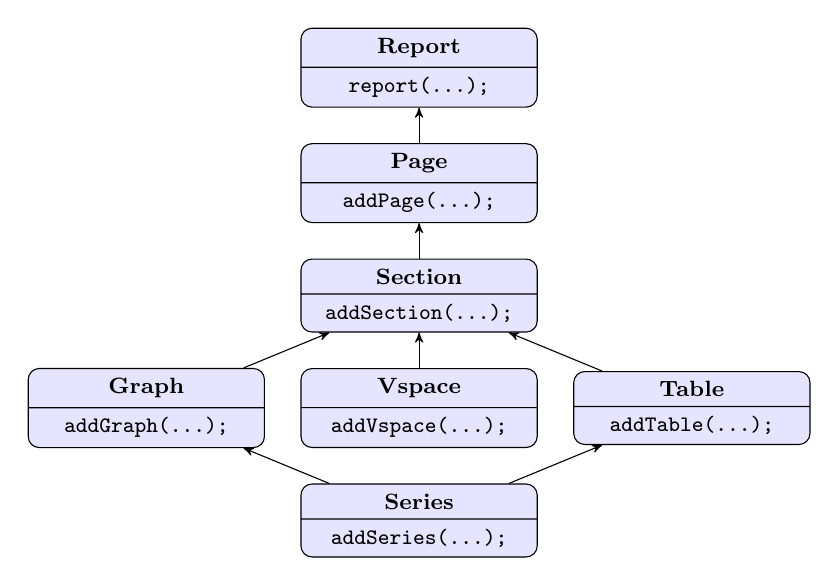
\begin{tikzpicture}[
        node distance = .45cm,
        auto,
        line/.style={->, >=stealth'},
      ]
      \node (Report) [abstract, rectangle split, rectangle split parts=2]
            {
              \textbf{Report}
              \nodepart{second}\texttt{report(...);}
            };
      \node (Page) [abstract, rectangle split, rectangle split parts=2, below=of Report]
            {
              \textbf{Page}
              \nodepart{second}\texttt{addPage(...);}
            };
      \node (Section) [abstract, rectangle split, rectangle split parts=2, below=of Page]
            {
              \textbf{Section}
              \nodepart{second}\texttt{addSection(...);}
            };
      \node (Vspace) [abstract, rectangle split, rectangle split parts=2, below=of Section]
            {
              \textbf{Vspace}
              \nodepart{second}\texttt{addVspace(...);}
            };
      \node (Graph) [abstract, rectangle split, rectangle split parts=2, left=of Vspace]
            {
              \textbf{Graph}
              \nodepart{second}\texttt{addGraph(...);}
            };
      \node (Table) [abstract, rectangle split, rectangle split parts=2, right=of Vspace, text height=]
            {
              \textbf{Table}
              \nodepart{second}\texttt{addTable(...);}
            };
      \node (Series) [abstract, rectangle split, rectangle split parts=2, below=of Vspace]
            {
              \textbf{Series}
              \nodepart{second}\texttt{addSeries(...);}
            };
      \draw [line] (Series) to node { } (Table);
      \draw [line] (Series) to node { } (Graph);
      \draw [line] (Table) to node { } (Section);
      \draw [line] (Graph) to node { } (Section);
      \draw [line] (Vspace) to node { } (Section);
      \draw [line] (Section) to node { } (Page);
      \draw [line] (Page) to node { } (Report);
    \end{tikzpicture}
  }
\end{frame}

\subsection{Syntax}


\subsection{Examples}


\section{Putting it All Together}

\end{document}
